\newpage

\section{Midterm 1 Review, Spring 2022}
Midterm Exam 1 will cover Chapters 1 -- 3 (except section 1.2 and the angle trisection part of 3.1) and activities 1 -- 18, some of which are on the schedule for this week.  We did not complete all of these activities in class so you will need to fill in some gaps.  
\subsection{Review Ideas}

\begin{itemize}\itemsep0em
\item Be able to state definitions of commonly used terms, such as 
\begin{itemize}
\item Perpendicular line, parallel line, line segment, ray, angle, circle
\item Concurrent, collinear
\item Equilateral, equiangular, and regular polygons
\item Acute, obtuse, and right angles and triangles; isosceles and scalene triangles
\item Straight, complementary, and supplementary angles
\item Trapezoid (inclusive and exclusive), parallelogram, rhombus, rectangle, square, kite
\item Median, perpendicular bisector, angle bisector, altitude
\item Centroid, circumcenter, incenter, orthocenter
\item Chord, arc, arc measure, central angle, inscribed angle, tangent
\end{itemize}
\item Be able to perform standard constructions and explain why they work. 
\item Be able to draw (careful) figures satisfying particular conditions.  
\item Be able to explain key concepts such as area and angle.   
\item Be able to state precisely the triangle congruence criteria. 
\item Know the properties of various special quadrilaterals and be able to prove them.  
\item Know the various centers of a triangle, how to construct them, and whether they can lie outside the triangle.  
\item Be able to state key theorems and prove them in at least two (2) ways, especially:  
\begin{itemize}
\item Isosceles triangle theorem and its converse
\item Pythagorean theorem and its converse
\item The angle sum of a triangle 
\end{itemize}
\end{itemize}

\subsection*{Review Problems}
\begin{prob}
Demonstrate and describe Euclid's (compass and straightedge) construction for an equilateral triangle.  Explain
why it works.\marginnote{What about a square or a regular hexagon?}
\end{prob}

\begin{prob}
Maddie had an idea for proving that the sum of the interior angles in a triangle is $180^\circ$:  Given $\triangle ABC$, draw a line through $C$ parallel to $\overline{AB}$.  Finish Maddie's proof.\marginnote{What were the approaches we used in class?}  
\[
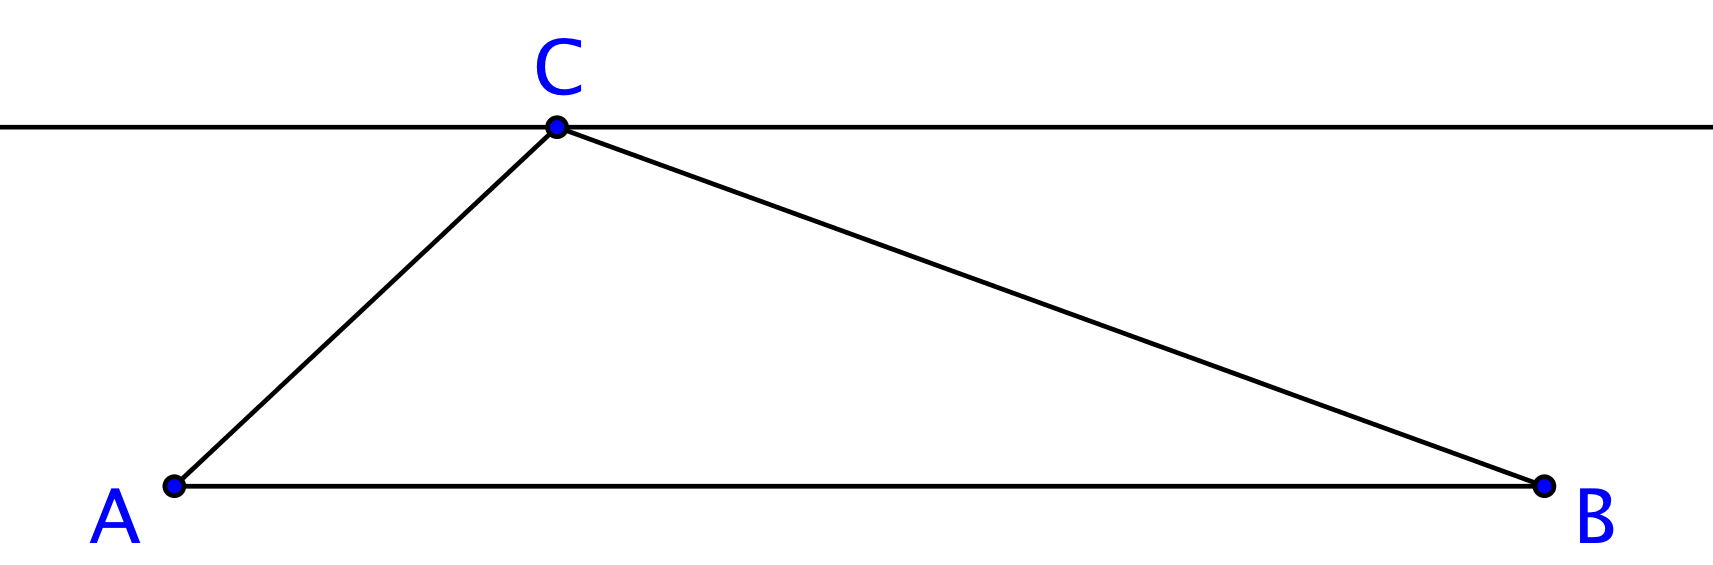
\includegraphics{../graphics/triangleAngleSum.png}
\]
\end{prob}

\begin{prob}
Use the picture below to show that a pair of medians intersects at a point 2/3 of the way from the vertex to the opposite side.  Then use that fact to argue that the three medians must be concurrent.
\[
\includegraphics[width=2.5in]{../graphics/median1.pdf}
\]
\end{prob}

\begin{prob}
Prove that the points on an angle bisector are \emph{exactly those} that are equidistant from the sides of the angle.\marginnote{What about the perpendicular bisectors?}
\end{prob}

\begin{prob}
Prove that the perpendicular bisectors of a triangle are concurrent.\marginnote[\baselineskip]{What about the angle bisectors?}
\end{prob}

\begin{prob}
Construct a $30$-$60$-$90$ right triangle. Explain the steps in your
 construction and how you know it works.\marginnote{What about a $45$-$45$-$90$ triangle?}
\end{prob}

%\begin{prob}
%Construct a $45$-$45$-$90$ right triangle. Explain the steps in your
%  construction and how you know it works.
%\end{prob}

\begin{prob}
Where is the orthocenter of a right triangle?  Explain your reasoning.  What about the circumcenter?  Again, explain your reasoning.\marginnote{What about the other centers of a right triangle?}
\end{prob}

\begin{prob}
Show that, given any three non-collinear points in the Euclidean plane, there is a unique circle passing through the three points.\marginnote{What about four points?}
\end{prob}

\begin{prob}
Construct a tangent line from a point outside a given circle to the circle.
\end{prob}

\begin{prob}
Give an informal derivation of the relationship between the circumference and area of a circle. 
\end{prob}

\begin{prob}
Complete the following statement:  When a quadrilateral is inscribed in a circle, opposite angles are \dots. 
Now prove the statement.  
\end{prob}

\begin{prob}
Claim:  A radius that is perpendicular to a chord bisects the chord.
\begin{enumerate}
\item Prove the claim.\marginnote{Use this problem structure for other problems.}
\item State the converse of the claim. 
\item Is the converse true?  If not, give a counterexample.  
\item If the converse is true, prove it.  If the converse is false, ``salvage it'' to make a true statement, and prove it.
\end{enumerate}
\end{prob}

\begin{prob}
State and prove the isosceles triangle theorem.\marginnote{What about the converse?}
\end{prob}

\begin{prob}
State and prove the Pythagorean theorem.\marginnote{What about the converse?}
\end{prob}

\begin{prob}
Prove any one of the following theorems about quadrilaterals.  State the converse of the theorem (regarding quadrilaterals).  If the converse is true, prove it.  If the converse is false, give a counterexample.  
\begin{enumerate}
\item Opposite sides of a parallelogram are congruent.
\item The diagonals of a rhombus are perpendicular.
\item The diagonals of a rectangle are congruent.
\item The diagonals of a parallelogram bisector each other.
\end{enumerate}
\end{prob}

\begin{prob}
Given a circle, describe a construction that finds its center.  Explain why it works.  
\end{prob}

\begin{prob}
Draw an arbitrary convex quadrilateral.  Form a second quadrilateral by connecting the 
midpoints of the sides of the first quadrilateral.  You will find that the second quadrilateral 
is a special quadrilateral.  Make a conjecture about the second quadrilateral and prove it.  
\end{prob}

%\begin{prob}
%The following picture shows a triangle that has been folded
%  along the dotted lines:
%\[
%\includegraphics{../graphics/origamiPBPTri.pdf}
%\]
%Explain how the picture ``proves'' the following statements:
%\begin{enumerate}
%\item The interior angles of a triangle sum to $180^\circ$. 
%\item The area of a triangle is given by $bh/2$. 
%\end{enumerate}
%\end{prob}
%
%\begin{prob}
%The figure below illustrates a construction given an angle $\theta$ and a segment $\overline{AB}$.  Line $\overleftrightarrow{DE}$ is the perpendicular bisector of $\overline{AB}$, and $\overleftrightarrow{BE}$ is perpendicular to $\overrightarrow{BC}$, as marked.  
%\[
%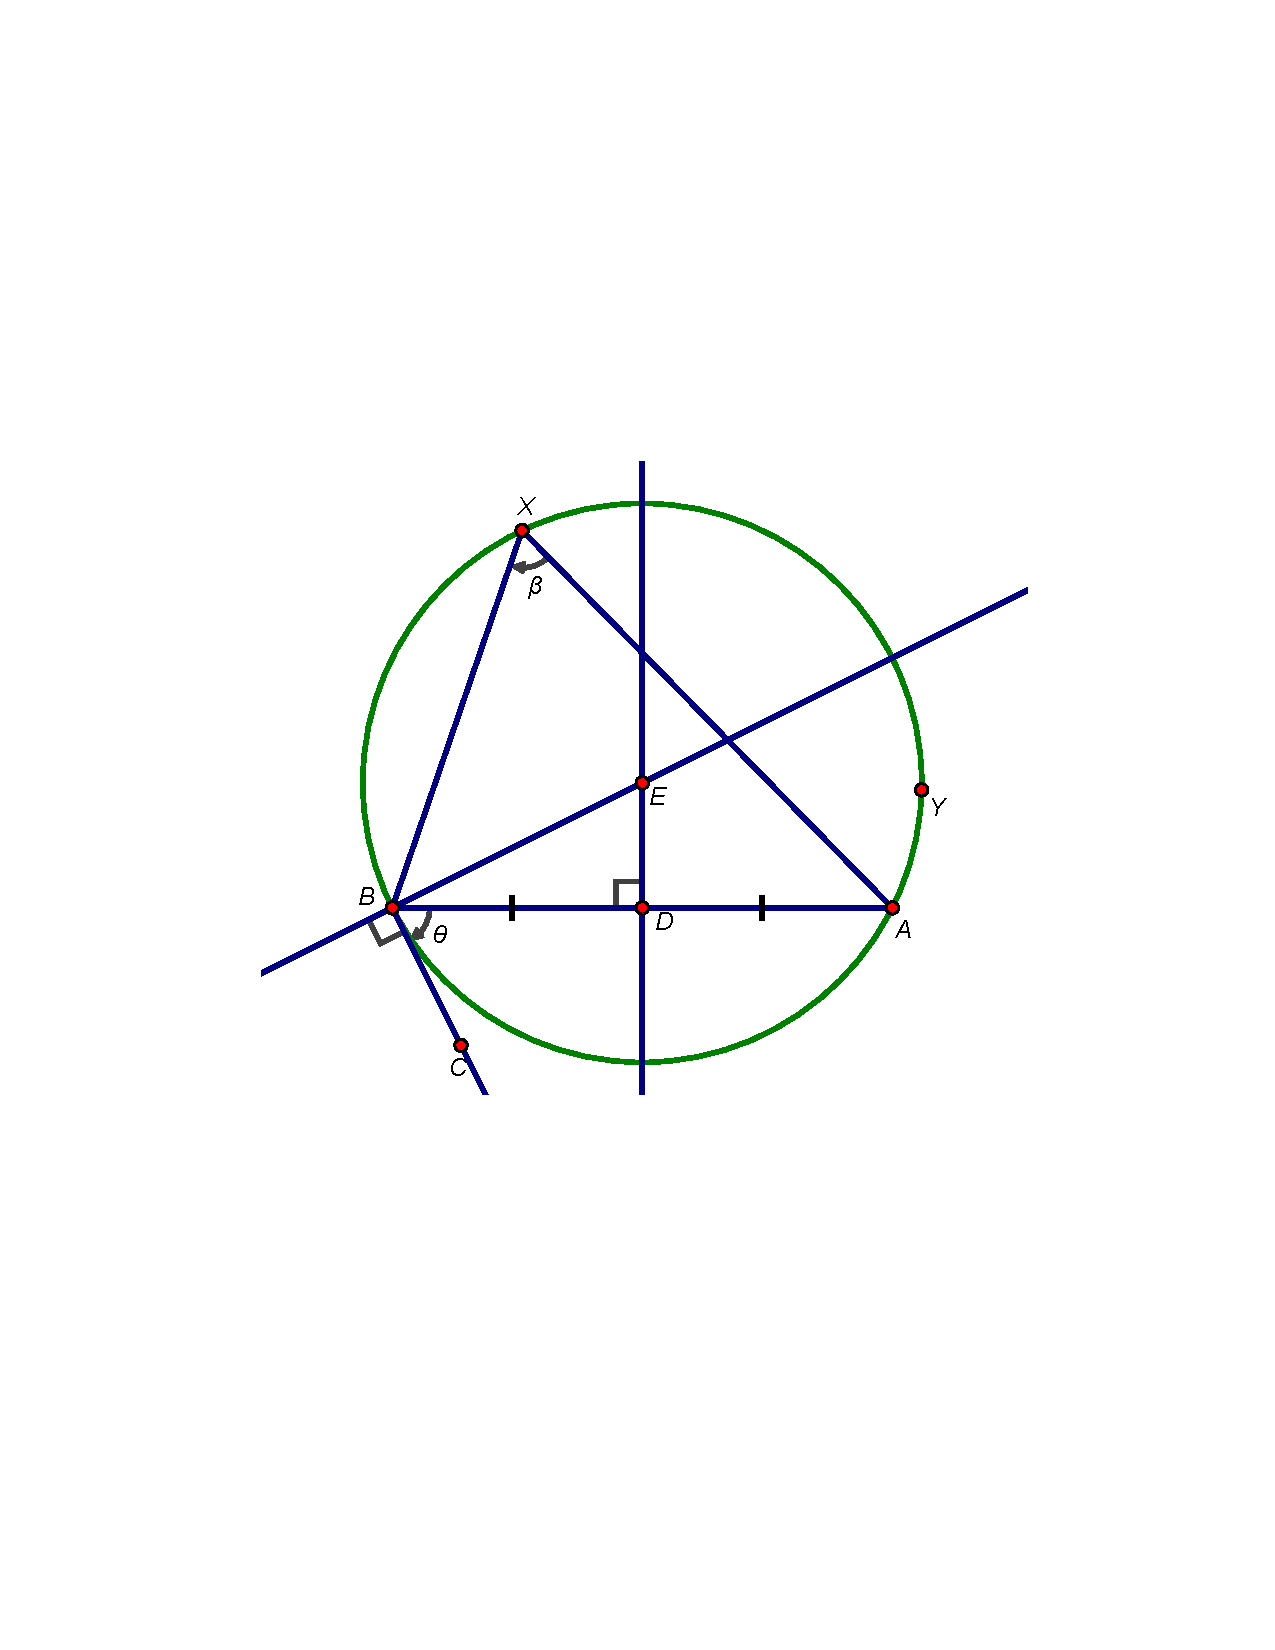
\includegraphics[scale=0.5]{../graphics/trickyConstruction}
%\]
%\begin{enumerate}
%%\item Mark the diagram and state what must be true about the construction so that $\angle\alpha=\angle\beta$. 
%\item Prove that $\angle\theta=\angle\beta$. 
%\item What will happen to $\angle\beta$ if point $X$ is moved over to point $Y$?  Say how you know.  
%\end{enumerate}
%\end{prob}